%%%%%%%%%%%%%%%%%%%%%%%%%%%%%%%%%%%%%%%%%%%%%%%%%%%%%%%%%%%%%%%%%%%%%%%%%%%%%%%
\section{Time needed for the momentum scale calibration with \piplusenu\ }
In this section we assume that a favorable S/B ratio can be achieved
and the \piplusenu\  scale calibration is possible, and estimate the time needed
for the calibration.

\begin{itemize}
\item 
  required accuracy of the momentum scale calibration : $\sigma_P/P$ < 100 keV ($@$100 MeV)
\item
  we consider scenario in which the momentum scale calibration is performed at two energies,
  50 MeV and B=0.5 T using the Michel edge and 70 MeV/c at B=0.7 T using \piplusenu\ decays
  of stopped positive pions. With the two measurements, one can extrapolate the momentum
  scale to the energy of 100 MeV. We note that a linear extrapolation would account
  for the first order non-linearity of the magnetic field.
\item
  extrapolation from 70 MeV to 100 MeV/c is a 30 MeV extrapolation,
  with the base being 70-50 = 20 MeV, as illustrated in Figure~\ref{figure:calibration_cartoon}
 
\begin{figure}[H]
  \begin{tikzpicture}
    \node[anchor=south west,inner sep=0] at (-0.2,0.) {
      % \node[shift={(0 cm,0.cm)},inner sep=0,rotate={90}] at (0,0) {}
      \makebox[\textwidth][c] {
        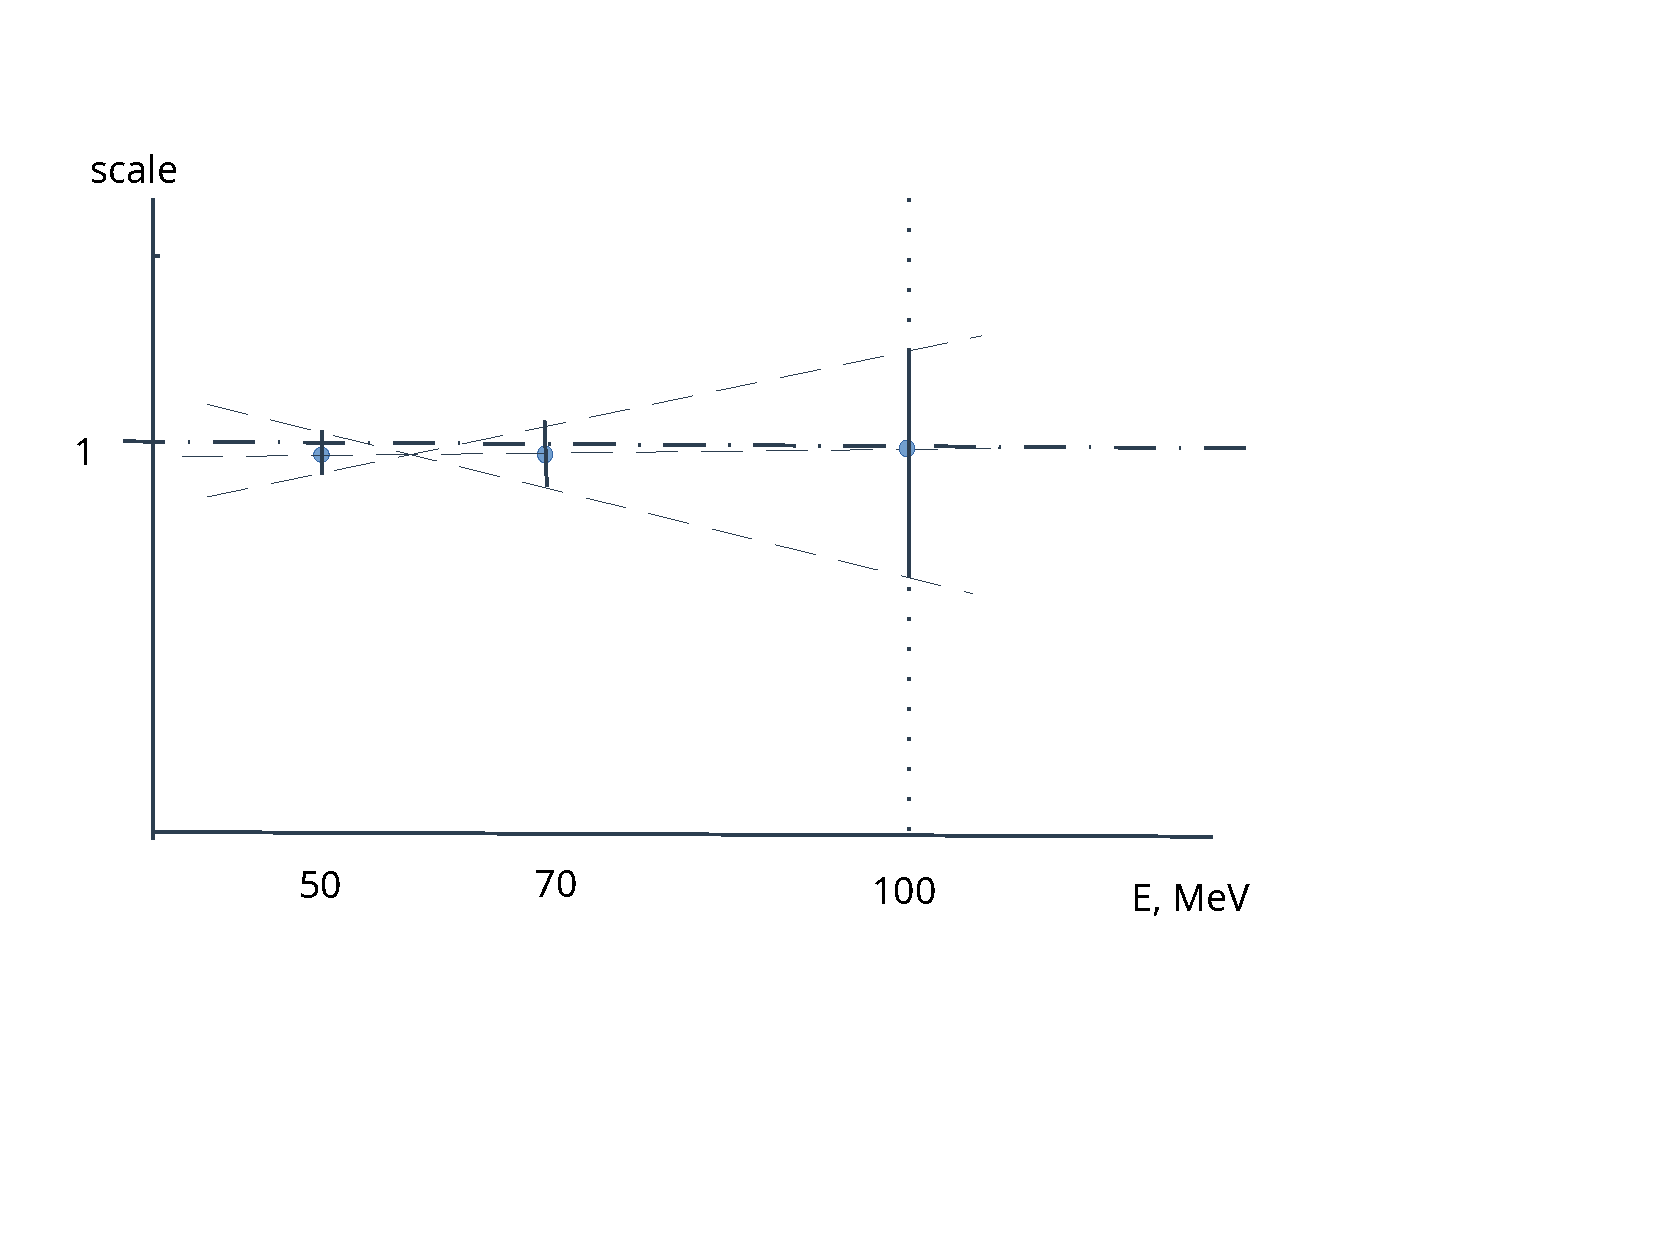
\includegraphics[width=0.8\textwidth]{pdf/momentum_scale_calibration}
      }
    };
    % \node [text width=8cm, scale=1.0] at (14.5,0.5) {$\mu_B$, expected background mean};
    % \node [text width=8cm, scale=1.0, rotate={90}] at (1.5,7.5) { $S_{D}$, ``discovery'' signal strength  };
  \end{tikzpicture}
  \caption{
    \label{figure:calibration_cartoon}
    Schematics of the momentum scale calibration
  }
\end{figure}
  
\item
  assuming perfect calibration at 50 MeV, uncertainty $\sigma_P/P$ $@$70 MeV translates
  into (30/20)$\sigma_P/P$, or $1.5\times(\sigma_P/P)@$100 MeV.
  Thus, the momentum scale at 70 MeV should be calibrated with an accuracy better
  than (100/1.5) MeV, say, $\sim$ 50 MeV.
\item
  FWHM of the \piplusenu\ momentum peak of 1 MeV/c translates into an estimate of
  $\sigma_P \sim 500$ keV, and 
  $$,
  \frac {500 {\rm ~keV}}{\sqrt N} <  50 {\rm ~keV} ~~
  $$
  or $N > 100$ events in the peak. We conservatively assume that the momentum scale calibration
  requires 1000 reconstructed \piplusenu\ events.
\item
  For a yield of $10^{-13}$ events/POT, collecting 1000 events requires $10^{16}$ protons on target.
\item
  in one-batch mode, an average expected pulse intensity is $1.6 \times 10^7$, and
  an average  pulse rate of 1$.6 \times 10^5$ pulses/sec gives the rate of $2.5 \times 10^{12}$ protons/sec.
\item
  Assuming running at 10\% of nominal beam intensity and the data collection efficiency of 50\%,
  collecting 1000 reconstructable \piplusenu\ events would require
  $10^{16}/(1.25 \times 10^{11}) \sim 10^5$ seconds, of about one day of running.
\item
  running at 10\% of nominal beam intensity with the digitization starting at 200 ns results in 
  the total number of background hits per microbunch of about 200, so the pileup at T>300 ns
  should not be a problem.
\end{itemize}

%%% Local Variables:
%%% mode: latex
%%% TeX-master: "mu2e-xxxxx"
%%% End:
